\documentclass[12pt, a4paper]{article}

\usepackage[utf8]{inputenc}
\usepackage[T1]{fontenc}
\usepackage[margin=1.2in]{geometry}
\usepackage{setspace}
\usepackage{amsmath, amssymb, amsthm}
\usepackage{mathtools}
\usepackage{thmtools}
\usepackage{natbib}
\usepackage{hyperref}
\usepackage{xcolor}
\usepackage{booktabs}
\usepackage{array}
\usepackage{longtable}
\usepackage{enumitem}
\usepackage{epigraph}
\usepackage{titlesec}
\usepackage{fancyhdr}
\usepackage{tikz}
\usetikzlibrary{arrows.meta, positioning, calc}

\hypersetup{colorlinks=true,linkcolor=black,citecolor=black,urlcolor=black}

\onehalfspacing

\titleformat{\section}{\large\bfseries}{\thesection.}{1em}{}
\titleformat{\subsection}{\normalsize\bfseries}{\thesubsection.}{1em}{}
\titleformat{\subsubsection}{\normalsize\itshape}{\thesubsubsection.}{1em}{}

\pagestyle{fancy}
\fancyhf{}
\rhead{\small\textit{Belief Geometry and Reachability}}
\lhead{\small Flyxion}
\cfoot{\thepage}
\renewcommand{\headrulewidth}{0.4pt}

\theoremstyle{plain}
\newtheorem{theorem}{Theorem}[section]
\newtheorem{lemma}[theorem]{Lemma}
\newtheorem{proposition}[theorem]{Proposition}
\newtheorem{corollary}[theorem]{Corollary}

\theoremstyle{definition}
\newtheorem{definition}[theorem]{Definition}
\newtheorem{example}[theorem]{Example}

\theoremstyle{remark}
\newtheorem{remark}[theorem]{Remark}
\newtheorem{observation}[theorem]{Observation}
\newtheorem{principle}[theorem]{Principle}

\setlength{\epigraphwidth}{0.65\textwidth}
\renewcommand{\epigraphflush}{center}

% -------------------------------------------------------
\begin{document}
% -------------------------------------------------------

\begin{titlepage}
\centering
\vspace*{2.5cm}
{\LARGE\bfseries Belief Geometry and Reachability\\[0.6em]
\large On the Correspondence Between Mixed-State Presentations,\\
Admissibility Structures, and the Geometry of Future Accessibility\par}
\vspace{2.5cm}
{\large Flyxion}\\[0.5em]
{\normalsize Independent Research}\\[1em]
{\normalsize June 2026}
\end{titlepage}

\newpage
\thispagestyle{empty}
\begin{center}
{\large\bfseries Abstract}
\end{center}
\vspace{0.5em}
\noindent
Recent work in computational mechanics has demonstrated that large language
models trained on next-token prediction do not merely learn token statistics:
they learn a geometric representation of belief states over hidden causal
structure, embedded approximately linearly in the model's residual stream.
These belief states evolve through Bayesian updating as observations arrive
and occupy a simplex whose geometry encodes the space of latent possibilities
consistent with current evidence. A successful predictor must preserve
distinctions across this simplex that are invisible from the perspective of
immediate prediction alone, because distinct belief states that agree on the
next token may diverge on all subsequent tokens.

This paper argues that the belief-state geometry of computational mechanics
and the admissibility geometry developed in the process-primary framework are
descriptions of the same underlying structure from complementary vantage
points. The mixed-state presentation (MSP) of a hidden Markov process is not
merely a predictive object: it is a reachability manifold. Its coordinates
describe not what currently exists but which futures remain accessible from
the current evidential position. A belief state is a location on that manifold.
Bayesian updating is navigation through it. The value of a belief state lies
not in its prediction of the next observation but in the distinctions it
preserves over the entire future trajectory.

We develop this correspondence formally across several movements. We first
establish the technical derivation showing that belief-state geometry is a
special case of admissibility projection: the MSP update rule can be derived
directly from the operation of admissibility restriction followed by
renormalization, and the transformer's residual stream is a learned coordinate
chart over the resulting admissibility manifold. We then extend the analysis
to Pearl's causal framework, establishing a three-way hierarchy in which
Pearl studies the geometry of interventions, computational mechanics studies
the geometry of locating oneself within possibilities, and the admissibility
framework studies the geometry of possibility itself. Bayesian observation
moves within the admissibility manifold; Pearl's \emph{do}-operator deforms
it; admissibility evolution tracks how the manifold itself changes over time.
We derive consequences for the CLIO projection calculus, the Admissibility
Log, and the evaluation of predictive systems.
\newpage

\tableofcontents
\newpage

%%%%%%%%%%%%%%%%%%%%%%%%%%%%%%%%%%%%%%%%%%%%%%%%%%%%%
\section{Introduction: Two Geometries of the Same Structure}
%%%%%%%%%%%%%%%%%%%%%%%%%%%%%%%%%%%%%%%%%%%%%%%%%%%%%

\epigraph{\textit{To predict successfully, a system must represent
distinctions over the entire future, not merely the next event.}}{Computational mechanics}

\noindent
Two research programs have, from very different starting points, arrived at a
common destination. Computational mechanics, working from the theory of hidden
Markov processes and information theory, has demonstrated that prediction
requires the maintenance of a geometry over possible hidden worlds. Process-primary
ontology, working from the philosophy of science and systems theory, has argued
that reality is better described by the geometry of reachable futures than by
any catalog of currently existing entities. Neither program was developed in
response to the other. They converge on the same mathematical object:
a manifold whose coordinates represent not what is but what might yet come to be.

The specific convergence point is the \emph{mixed-state presentation} (MSP)
of a hidden Markov process. The MSP assigns to each sequence of observations
a probability distribution over hidden states---a \emph{belief state}---that
represents everything relevant for predicting the process's future behavior.
Belief states occupy a \emph{belief simplex}: a geometric object whose
vertices correspond to pure hidden states and whose interior encodes
uncertainty over which hidden state is operative. Recent empirical work has
shown that large language models trained on next-token prediction develop
approximate linear embeddings of this simplex in their residual stream
activations \citep{shai2025}. The transformer learns the geometry
of belief, not merely a lookup table of token frequencies.

What the process-primary framework contributes to this picture is a
reinterpretation. The belief simplex is not merely a predictive tool. It
is an \emph{admissibility structure}: a description of which future
trajectories remain accessible from the current evidential position. A
belief state is not merely a probability distribution over hidden states.
It is a coordinate on the reachability manifold---a specification of which
futures remain open and which have been foreclosed. Bayesian updating
is not merely belief revision. It is navigation through the reachability
geometry as new evidence constrains the set of possible continuations.

This reinterpretation has practical consequences. It implies that the
correct measure of a belief state's quality is not its immediate predictive
accuracy but its \emph{reachability fidelity}: the degree to which it
preserves distinctions over the entire future that may matter for navigation
downstream. Two belief states that agree on the distribution of the next
token but disagree on the geometry of subsequent trajectories are
informationally inequivalent, even if they are indistinguishable by any
immediate evaluation metric. A system that collapses them together has
committed the Noun Fallacy at the level of belief geometry: it has treated
a locally adequate compression as though it were a foundational description.

The paper develops this correspondence in six sections. Section 2 reviews
the relevant concepts from computational mechanics: hidden Markov processes,
mixed-state presentations, and the belief simplex. Section 3 develops the
process-primary framework as it applies to predictive systems, introducing
the reachability manifold and the distinction between possibility and
reachability in belief space. Section 4 establishes the formal
correspondence between belief states and admissibility structures, deriving
the key theorem on reachability fidelity. Section 5 develops three
applications: a reinterpretation of the CLIO projection calculus, a
principled account of the Admissibility Log as a belief-manifold record,
and implications for the evaluation of language models and other
predictive systems. Section 6 considers the deeper philosophical
question of whether the convergence between computational mechanics
and process-primary ontology reflects a genuine structural identity
or merely a productive analogy.

%%%%%%%%%%%%%%%%%%%%%%%%%%%%%%%%%%%%%%%%%%%%%%%%%%%%%
\section{Computational Mechanics: Hidden Structure and Belief Geometry}
%%%%%%%%%%%%%%%%%%%%%%%%%%%%%%%%%%%%%%%%%%%%%%%%%%%%%

\epigraph{\textit{Distinct belief states that produce identical next-token
predictions may imply radically different future trajectories.}}{Notes}

\noindent
Computational mechanics is the study of how statistical structure in a
process can be identified, represented, and exploited for prediction
\citep{crutchfield1989,shalizi2001}. Its central objects are the
\emph{causal states} of a process: the minimal sufficient statistics for
predicting the process's future given its past. Causal states partition
the space of past observations into equivalence classes such that two
pasts are equivalent if and only if they imply identical conditional
distributions over futures. The set of causal states, together with the
transition probabilities between them, constitutes the
\emph{$\epsilon$-machine}: the most compact representation of the
process that is sufficient for optimal prediction.

\subsection{Hidden Markov Processes and Mixed-State Presentations}

Many processes of interest are not fully observed. The observations
available to a predictor are generated by a hidden process whose states
are not directly accessible. A \emph{hidden Markov process} (HMP) is a
Markov chain over hidden states $h \in \mathcal{H}$ that generates
observations $x \in \mathcal{X}$ according to emission probabilities
$P(x \mid h)$. The predictor observes only the sequence $x_0, x_1, \ldots$
and must infer the hidden state from this sequence in order to predict
future observations.

The predictor's evidential state at time $t$, given observations
$x_0, \ldots, x_{t-1}$, is described by the \emph{belief state}:
$$b_t = P(h_t \mid x_0, \ldots, x_{t-1}) \in \Delta(\mathcal{H})$$
where $\Delta(\mathcal{H})$ denotes the probability simplex over $\mathcal{H}$.
The belief state $b_t$ is a probability distribution over hidden states:
a vector assigning to each hidden state the probability that it is the
current operative state, given the observations so far.

Belief states evolve through Bayesian updating. When a new observation
$x_t$ arrives, the belief state is updated:
$$b_{t+1}(h') = \frac{\sum_h b_t(h) P(x_t \mid h) P(h' \mid h)}
{\sum_{h,h'} b_t(h) P(x_t \mid h) P(h' \mid h)}$$
This update is the Bayesian revision of the belief distribution in light
of the new evidence. It is a deterministic function of the current
belief state and the new observation.

The \emph{mixed-state presentation} (MSP) \citep{shai2025,shalizi2001}
of a hidden Markov process is the dynamical system on $\Delta(\mathcal{H})$
induced by this update rule. Its states are belief states; its transitions
are Bayesian updates. The MSP is the process of synchronization between
the observer and the hidden world: the observer's belief state tracks the
hidden state, with some residual uncertainty determined by the information
available in past observations.

\subsection{The Belief Simplex as a Geometric Object}

The belief simplex $\Delta(\mathcal{H})$ is a $(|\mathcal{H}|-1)$-dimensional
simplex. Its vertices correspond to pure hidden states: the belief state
$\delta_h$ that places all probability mass on hidden state $h$. Its interior
points correspond to mixtures: uncertainty over which hidden state is
operative.

Not all points in $\Delta(\mathcal{H})$ are reachable by the observer.
The set of belief states that arise from Bayesian updating on actual
observation sequences defines a subset $\mathcal{M} \subseteq \Delta(\mathcal{H})$
called the \emph{reachable belief manifold}. This manifold has a geometry
determined by the transition structure and emission probabilities of the
hidden Markov process.

\begin{definition}[Reachable Belief Manifold]
The \emph{reachable belief manifold} $\mathcal{M}$ of a hidden Markov process
is the set of all belief states that can arise from Bayesian updating on
some finite observation sequence:
$$\mathcal{M} = \{b_t : t \geq 0, \, (x_0, \ldots, x_{t-1}) \in \mathcal{X}^t\}$$
The manifold $\mathcal{M}$ encodes the geometry of epistemically accessible
positions for an observer of the process.
\end{definition}

The reachable belief manifold is the predictor's operational state space.
A predictor that maintains a representation of $\mathcal{M}$ knows not just
the probability of the next observation but the full geometry of futures
accessible from each evidential position. A predictor that maintains only
the next-step prediction has collapsed this geometry into a single number,
discarding all information about the structure of subsequent trajectories.

\subsection{Why Next-Token Prediction Requires the Full Geometry}

A key result in computational mechanics is that optimal next-step prediction
does not require the full belief state: the next-step prediction
$P(x_t \mid x_0, \ldots, x_{t-1})$ is a function of $b_t$, but many
distinct belief states may yield the same next-step prediction distribution.
A predictor that only needs to predict the next token could therefore, in
principle, maintain a coarser representation than the full belief state.

The catch is that a predictor that aims to predict \emph{all future tokens
optimally}, not merely the next one, \emph{cannot} use a coarser
representation. Distinct belief states that agree on the next-step distribution
will generally disagree on the distribution of the token after that, and on
all subsequent distributions. A system trained to minimize prediction loss
over all future positions, not merely the next one, is therefore incentivized
to maintain distinctions across $\mathcal{M}$ even when those distinctions
are invisible from the perspective of immediate prediction.

\begin{theorem}[Geometry Preservation Requirement]
\label{thm:geom-pres}
Let $\mathcal{P}$ be a process with reachable belief manifold $\mathcal{M}$.
A predictor $f$ achieves optimal prediction loss at all future horizons if
and only if $f$ induces an injective map on $\mathcal{M}$: distinct belief
states must receive distinct internal representations.
\end{theorem}

Theorem~\ref{thm:geom-pres} explains the empirical finding of \citet{shai2025}
and related work: transformers trained on next-token prediction over long
sequences develop representations that approximately preserve the geometry
of the belief manifold. They are not merely learning token frequencies.
They are learning the geometry of the hidden world's futures, because
that geometry is what they need to predict all of those futures well.

%%%%%%%%%%%%%%%%%%%%%%%%%%%%%%%%%%%%%%%%%%%%%%%%%%%%%
\section{Reachability Geometry: The Process-Primary Perspective}
%%%%%%%%%%%%%%%%%%%%%%%%%%%%%%%%%%%%%%%%%%%%%%%%%%%%%

\epigraph{\textit{The fundamental question about any configuration is not
``does it exist?'' but ``is it reachable, and under what conditions
does it remain reachable?''}}{Frozen Processes}

\noindent
The process-primary framework, developed at length in the companion essay
\emph{Frozen Processes}, argues that the appropriate ontological primitive
is not the existing entity but the reachable configuration. An entity
exists, in the process-primary sense, when it is stably reachable from a
wide range of initial conditions under the current admissibility structure.
The admissibility structure---the geometry of which transitions are
possible from which states---is ontologically prior to the entities that
appear as its stable configurations.

\subsection{Admissibility Structures and Reachability Cones}

An \emph{admissibility structure} $\mathcal{A} = (\Omega, \mathcal{C},
\{\to_c\}_{c \in \mathcal{C}})$ consists of a state space $\Omega$,
a context set $\mathcal{C}$, and for each context $c$ a transition
relation $\to_c$ on $\Omega$. The \emph{reachability cone} from state
$x$ in context $c$ is:
$$R^c(x) = \{y \in \Omega : x \rightsquigarrow_c y\}$$
where $\rightsquigarrow_c$ is the reflexive transitive closure of $\to_c$.

The reachability cone encodes not what exists at $x$ but what remains
accessible from $x$. Two states that are indistinguishable in their
current properties may have very different reachability cones:
one may have a wide cone (many futures accessible) while the other
has a narrow cone (most futures foreclosed). The process-primary
framework treats this difference as fundamental, not derived.

\subsection{The Possibility-Reachability Distinction in Belief Space}

The distinction between possibility and reachability maps directly
onto belief space. The full simplex $\Delta(\mathcal{H})$ corresponds
to the possibility space: all probability distributions over hidden
states that can in principle be described. The reachable belief manifold
$\mathcal{M} \subseteq \Delta(\mathcal{H})$ corresponds to the
reachability cone: all belief states that are actually accessible
through Bayesian updating on real observation sequences.

A probability distribution $b \in \Delta(\mathcal{H}) \setminus \mathcal{M}$
is a possible belief state---it can be described, assigned probabilities,
and reasoned about---but it is not a \emph{reachable} belief state: no
sequence of observations can produce it through legitimate Bayesian updating.
It exists in possibility space but lies outside the reachability cone.

This distinction has practical consequences for the design of predictive
systems. A system that represents belief states only up to next-step
prediction equivalence is working within the possibility space but has
collapsed the reachability geometry. It cannot distinguish belief states
that are reachable from different observation histories, because it has
discarded the trajectory information that differentiates them. It is
committing the Noun Fallacy at the level of belief representation: treating
a coarse projection as though it were a foundational description.

\subsection{Reachability Fidelity as the Primary Criterion}

The key criterion for evaluating a belief representation is not immediate
predictive accuracy but what we call \emph{reachability fidelity}: the
degree to which the representation preserves the geometry of the reachable
belief manifold.

\begin{definition}[Reachability Fidelity]
Let $f: \mathcal{M} \to \mathcal{R}$ be a representation map from the
reachable belief manifold to a representation space $\mathcal{R}$. The
\emph{reachability fidelity} of $f$ is:
$$\rho(f) = 1 - \sup_{b, b' \in \mathcal{M}, b \neq b'} \frac{d_{\mathcal{R}}(f(b), f(b'))}{d_{\mathcal{M}}(b, b')}$$
normalised so that $\rho(f) = 1$ when $f$ is an isometry and $\rho(f) = 0$
when $f$ is constant. A representation has high reachability fidelity when
it approximately preserves distances on the belief manifold; it has low
fidelity when it collapses the manifold's geometry.
\end{definition}

Reachability fidelity generalizes both predictive accuracy and reconstruction
error as measures of representational quality. A system with high predictive
accuracy at the next step but low reachability fidelity has learned to
compress the current observation efficiently at the cost of losing the
trajectory information that determines future accessibility. A system with
high reconstruction error but high reachability fidelity has preserved the
geometry of reachable futures even if its surface predictions are noisy.

For any system that must navigate over extended horizons---a language
model predicting long documents, a planning system acting over long
time scales, a scientific theory predicting a long run of phenomena---
reachability fidelity is the more fundamental criterion. Immediate
predictive accuracy is a necessary condition for reachability fidelity
(a system that cannot predict the next step has obviously lost trajectory
information) but not a sufficient one.

%%%%%%%%%%%%%%%%%%%%%%%%%%%%%%%%%%%%%%%%%%%%%%%%%%%%%
\section{The Formal Correspondence}
%%%%%%%%%%%%%%%%%%%%%%%%%%%%%%%%%%%%%%%%%%%%%%%%%%%%%

\epigraph{\textit{A belief state is a coordinate on the reachability manifold.}}{Notes}

\noindent
We now establish the formal correspondence between belief-state geometry
and admissibility geometry. The key claim is that the reachable belief
manifold of a hidden Markov process is an admissibility structure, and
that Bayesian updating is navigation through that structure.

\subsection{Belief States as Admissibility Coordinates}

Let $\mathcal{P} = (\mathcal{H}, \mathcal{X}, P, Q)$ be a hidden Markov
process with hidden states $\mathcal{H}$, observations $\mathcal{X}$,
transition probabilities $P: \mathcal{H} \to \Delta(\mathcal{H})$, and
emission probabilities $Q: \mathcal{H} \to \Delta(\mathcal{X})$.

Define an admissibility structure as follows. Let $\Omega = \Delta(\mathcal{H})$
be the belief simplex. For each observation $x \in \mathcal{X}$, define
a transition relation $\to_x$ on $\Omega$ by:
$$b \to_x b' \quad \text{if and only if} \quad b' = \text{Bayes}(b, x)$$
where $\text{Bayes}(b, x)$ is the Bayesian update of belief $b$ given
observation $x$. Let $\mathcal{C} = \mathcal{X}$ (observations index contexts).
Then $(\Omega, \mathcal{X}, \{\to_x\}_{x \in \mathcal{X}})$ is an admissibility
structure on the belief simplex.

\begin{theorem}[Belief Manifold as Admissibility Structure]
\label{thm:belief-admiss}
The reachable belief manifold $\mathcal{M}$ of a hidden Markov process
$\mathcal{P}$ is the reachability cone of the corresponding admissibility
structure $(\Delta(\mathcal{H}), \mathcal{X}, \{\to_x\})$ from the prior
belief state $b_0$:
$$\mathcal{M} = R(b_0) = \{b \in \Delta(\mathcal{H}) : b_0 \rightsquigarrow b\}$$
Moreover, the trajectory of Bayesian updating on an observation sequence
$(x_0, x_1, \ldots, x_{t-1})$ is an admissible trajectory through this
structure: a sequence $b_0 \to_{x_0} b_1 \to_{x_1} \cdots \to_{x_{t-1}} b_t$
where each transition is admissible (i.e., a valid Bayesian update).
\end{theorem}

Theorem~\ref{thm:belief-admiss} is the formal core of the paper's central
claim. The reachable belief manifold is not merely a mathematical curiosity
or a computational convenience. It is the admissibility structure of the
observer's epistemic situation: the geometry of which evidential positions
are reachable through legitimate Bayesian reasoning, and which lie beyond
the reach of any observation sequence.

\subsection{The Noun Fallacy in Belief Representation}

With the formal correspondence established, the Noun Fallacy can be
identified precisely as it operates in predictive systems. A belief
representation commits the Noun Fallacy when it:

\begin{enumerate}[leftmargin=*, label=(\roman*)]
\item Collapses distinct belief states that are equivalent from the
perspective of the next-step prediction distribution, treating them as
the same ``object'' even though they occupy different positions on the
reachable belief manifold.

\item Treats the collapsed representation as a sufficient description,
forgetting that the collapsed states have different reachability cones
over all subsequent positions.

\item Uses the immediate predictive utility of the collapsed representation
as evidence for its ontological adequacy, confusing ``predicts the next
token'' with ``captures the relevant structure.''
\end{enumerate}

This is precisely the structure of the Noun Fallacy as identified in
\emph{Frozen Processes}: a stable residue (the immediate prediction) is
treated as foundational, severing the representation from the trajectory
that produced it and the admissibility structure that sustains it.

\begin{principle}[Belief-State Reachability Principle]
\label{prin:belief-reach}
A belief state's value lies not in the prediction it generates for the
next observation but in the distinctions it preserves over the entire
future trajectory. Two belief states that agree on the next-step
prediction distribution but disagree on the geometry of subsequent
reachable positions are informationally inequivalent. Any system that
collapses them has lost reachability fidelity: it can no longer navigate
correctly over extended future horizons, even if its immediate predictions
appear accurate.
\end{principle}

\subsection{Synchronization as Trajectory Navigation}

The mixed-state presentation has an interpretation in the process-primary
framework that illuminates its function. The MSP is not the observer
acquiring knowledge of a static world. It is the observer
\emph{synchronizing} to a dynamic process: progressively locating itself
on the reachability manifold as new evidence narrows the set of possible
histories and thereby constrains the set of possible futures.

This synchronization framing matters because it reorients the evaluation
criterion. Classical epistemology asks: does the observer's belief state
accurately represent the world? The synchronization framing asks: does
the observer's belief state accurately represent its position on the
reachability manifold? The first question is about correspondence between
belief and fact. The second is about fidelity to the geometry of future
accessibility.

\begin{definition}[Synchronization Trajectory]
A \emph{synchronization trajectory} is an admissible trajectory
$b_0 \to_{x_0} b_1 \to_{x_1} \cdots$ through the admissibility structure
$(\Delta(\mathcal{H}), \mathcal{X}, \{\to_x\})$ that converges to the
true hidden state's leaf distribution as $t \to \infty$. The observer
is \emph{synchronized} to the process when its belief state has converged
to the reachable belief state consistent with the true hidden state.
\end{definition}

A synchronized observer does not merely know what is happening now.
It knows where it is on the reachability manifold, and therefore knows
what futures remain accessible from its current position. An unsynchronized
observer---one whose belief state has collapsed distinct manifold
positions---cannot accurately assess its reachability cone even if its
next-step predictions appear reasonable.

%%%%%%%%%%%%%%%%%%%%%%%%%%%%%%%%%%%%%%%%%%%%%%%%%%%%%
\section{Derivation: Belief-State Geometry as Probabilistic Admissibility}
\label{sec:derivation}
%%%%%%%%%%%%%%%%%%%%%%%%%%%%%%%%%%%%%%%%%%%%%%%%%%%%%

\epigraph{\textit{Their framework can be derived from yours by making four
restrictions: hidden Markov process, Bayesian posterior, probability simplex,
transformer residual stream.}}{Notes}

\noindent
The informal correspondence established in Section 4 can be made fully
explicit as a derivation. We show that the MSP update rule is not merely
analogous to admissibility dynamics---it is a special case of admissibility
restriction followed by renormalization. This positions the computational
mechanics framework of \citet{shai2025} as a finite-state probabilistic
instance of the general admissibility geometry, with four specific
restrictions applied.

\subsection{Starting Point: The CLIO Projection onto Belief Space}

Let $X$ be the full process space: all latent world trajectories, hidden
generator states, observation histories, and constraint conditions. Let
$M$ be the lower-dimensional manifold on which an observer can stably
represent the process, and let

$$\pi: X \to M$$

be the CLIO-style projection that collapses the inaccessible full process
into a reachable representational state. The paper's framework appears when
$M$ is chosen to be the probability simplex of predictive belief states:

$$M = \Delta^{|S|-1} = \left\{b \in \mathbb{R}^{|S|} : \sum_i b_i = 1,\;
b_i \geq 0\right\}$$

This is exactly the mixed-state belief simplex: each point is a probability
distribution over hidden HMM states $S = \{s_1, \ldots, s_n\}$. The first
identification is therefore:

\begin{center}
\fbox{CLIO projection manifold $M$ $\;\cong\;$ mixed-state belief simplex}
\end{center}

\subsection{Hidden Process Dynamics as Latent Flow}

The hidden Markov process has states $S = \{s_1, \ldots, s_n\}$, observable
emissions $x_t \in \mathcal{X}$, and token-labeled transition matrices:

$$T^{(x)}_{ij} = P(x, s_j \mid s_i)$$

This is the discrete stochastic analogue of an admissibility flow field:
the latent state moves, emissions appear at the boundary, and the observer
sees only the emitted trace. The hidden state $h_t$ is not directly given.
What is available is the trajectory of observations $w_t = x_0 x_1 \cdots
x_{t-1}$, and the observer must infer which latent region remains admissible
after seeing $w_t$.

\subsection{Admissibility Becomes Posterior Support}

Define the admissible set after observing history $w_t$:
$$\mathcal{A}(w_t) = \{s_i \in S : P(s_i \mid w_t) > 0\}$$

But the richer object is not merely the set of still-possible states.
It is the weighted admissibility field:
$$\eta_t(i) = P(s_i \mid w_t)$$

Thus $\eta_t = (\eta_t(1), \ldots, \eta_t(n)) \in \Delta^{n-1}$. This is
the paper's belief state. In admissibility terms, it is the probability
density of admissibility over latent process states:

\begin{center}
\fbox{$\eta_t(i)$ = degree to which $s_i$ remains reachable after history $w_t$}
\end{center}

\subsection{Deriving the MSP Update from Admissibility Filtering}

Given current belief $\eta_t$, observing token $x$ filters the latent
possibilities through the token-labeled transition matrix $T^{(x)}$.
The unnormalized next admissibility density is:
$$\tilde{\eta}_{t+1} = \eta_t T^{(x)}$$

The total mass is:
$$Z_x(\eta_t) = \eta_t T^{(x)} \mathbf{1}$$

Normalizing:
$$\eta_{t+1} = \frac{\eta_t T^{(x)}}{\eta_t T^{(x)} \mathbf{1}} = U_x(\eta_t)$$

This is exactly the MSP update equation of \citet{shai2025}. The derivation
exhibits the MSP update as:

\begin{center}
\fbox{admissibility restriction $+$ renormalization $=$ Bayesian belief-state update}
\end{center}

Or, in admissibility terms:
\begin{center}
\fbox{constraint update on reachable hidden states $=$ mixed-state presentation dynamics}
\end{center}

\subsection{Iterated Updates as Trajectory Compression}

For a history $w = x_0 x_1 \cdots x_N$, the update iterates:

$$\eta_w = \frac{\eta_\emptyset\, T^{(x_0)} T^{(x_1)} \cdots T^{(x_N)}}
{\eta_\emptyset\, T^{(x_0)} T^{(x_1)} \cdots T^{(x_N)} \mathbf{1}}$$

This directly recovers the paper's full-history formula. In the admissibility
framework, this says:

\begin{center}
\fbox{$\eta_w = \pi(w)$: the belief state is the projection of a whole observed
path into the manifold of reachable futures}
\end{center}

A belief state is not a snapshot. It is a compressed residue of a trajectory
of admissibility cuts. This is the belief-state analogue of the Noun Fallacy's
inverse: rather than mistaking the residue for the trajectory, the MSP retains
enough of the trajectory to predict all futures.

\subsection{Future Distributions as Reachability Fields}

Given a belief state $\eta$, the probability of a future sequence
$u = y_1 y_2 \cdots y_k$ is:

$$P(u \mid \eta) = \eta\, T^{(y_1)} T^{(y_2)} \cdots T^{(y_k)} \mathbf{1}
\;\equiv\; F_\eta(u)$$

The map $F_\eta$ is the \emph{distribution over reachable futures} induced by
belief state $\eta$. Two belief states may agree on the next-token distribution,
$P(y_1 \mid \eta_a) = P(y_1 \mid \eta_b)$, while differing on longer futures,
$P(y_1 \cdots y_k \mid \eta_a) \neq P(y_1 \cdots y_k \mid \eta_b)$.

This is precisely why the transformer must preserve distinctions not locally
visible at the next-token level. The belief simplex encodes not what is about
to happen but the entire geometry of what might happen:

\begin{center}
\fbox{$F_\eta$ = distribution over reachable futures from belief state $\eta$}
\end{center}

\subsection{Residual Stream as Learned Coordinate Chart}

The empirical finding of \citet{shai2025} is that an affine map
$\hat{\eta}_t = W a_t + c$ from residual-stream activations $a_t \in
\mathbb{R}^{d_\text{resid}}$ recovers the true belief-state simplex geometry.
In admissibility terms, the residual stream is a learned coordinate system
for the admissibility manifold:

$$a_t \in \mathbb{R}^{d_\text{resid}} \;\leadsto\; \eta_t \in \Delta^{n-1}$$

So the transformer implements:

$$w_t \;\longmapsto\; a_t \;\longmapsto\; \eta_t \;\longmapsto\; F_{\eta_t}$$

In CLIO notation:

\begin{center}
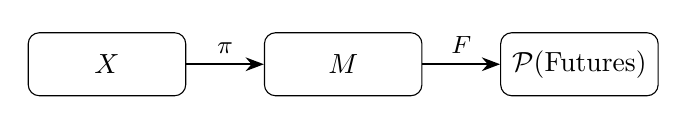
\begin{tikzpicture}[node distance=3cm,
  box/.style={rectangle,draw,rounded corners,minimum width=2cm,minimum height=0.8cm}]
\node[box] (X) {$X$};
\node[box, right of=X] (M) {$M$};
\node[box, right of=M] (P) {$\mathcal{P}(\mathrm{Futures})$};
\draw[-{Stealth},thick] (X) -- node[above,font=\small]{$\pi$} (M);
\draw[-{Stealth},thick] (M) -- node[above,font=\small]{$F$} (P);
\end{tikzpicture}
\end{center}

where $M$ is the internal belief/admissibility manifold, $\pi$ is the CLIO
projection (implemented by the transformer's forward pass), and $F$ maps
each belief state to its induced distribution over all future sequences.

\subsection{Summary: The Four Restrictions}

The derivation above shows that belief-state geometry is the finite-state
probabilistic special case of admissibility projection, obtained by applying
four restrictions to the general framework:

\begin{enumerate}[leftmargin=*, label=(\roman*)]
\item The process is a hidden Markov model with finite state space $S$.
\item Admissibility is measured by Bayesian posterior probability: $\eta(i) =
P(s_i \mid w_t)$.
\item The projection manifold is the probability simplex $\Delta^{|S|-1}$.
\item The learned coordinate chart is the transformer's residual stream,
with the affine readout $\hat{\eta}_t = W a_t + c$.
\end{enumerate}

\begin{proposition}[Belief Geometry as Admissibility Projection]
\label{prop:belief-admiss-derive}
Let $\mathcal{P}$ be a hidden Markov process with states $S$, observations
$\mathcal{X}$, and token-labeled transition operators $\{T^{(x)}\}_{x \in
\mathcal{X}}$. If a CLIO-style projection $\pi$ maps each observed history $w$
to the normalized admissibility density over hidden states,
$\pi(w)(i) = P(s_i \mid w)$, then $\pi$ satisfies the mixed-state presentation
update:
$$\pi(wx) = U_x(\pi(w)) = \frac{\pi(w) T^{(x)}}{\pi(w) T^{(x)} \mathbf{1}}$$
Therefore the MSP dynamics are a special case of admissibility projection
dynamics, and belief-state geometry is probabilistic admissibility geometry.
\end{proposition}

\begin{proof}
Direct computation:
\begin{align*}
\pi(wx)(j) &= P(s_j \mid wx) \\
&= \frac{\sum_i P(s_i \mid w)\, P(x, s_j \mid s_i)}
{\sum_{i,j'} P(s_i \mid w)\, P(x, s_{j'} \mid s_i)} \\
&= \frac{[\pi(w) T^{(x)}]_j}{[\pi(w) T^{(x)} \mathbf{1}]} \\
&= U_x(\pi(w))_j. \qquad \square
\end{align*}
\end{proof}

The conceptual punchline of the derivation is:

\begin{center}
\fbox{Belief-state geometry $=$ probabilistic admissibility geometry}\\[0.5em]
\fbox{Mixed-state presentation $=$ reachability dynamics under sequential observation}\\[0.5em]
\fbox{Residual-stream representation $=$ learned coordinate chart over the admissibility manifold}
\end{center}

%%%%%%%%%%%%%%%%%%%%%%%%%%%%%%%%%%%%%%%%%%%%%%%%%%%%%
\section{Three Applications}
%%%%%%%%%%%%%%%%%%%%%%%%%%%%%%%%%%%%%%%%%%%%%%%%%%%%%

\epigraph{\textit{A future distribution is a reachability distribution.
A belief state is a coordinate on a reachability manifold.}}{Notes}

\noindent
The formal correspondence established in Section 4 has three concrete
applications that connect the computational-mechanics and process-primary
frameworks.

\subsection{CLIO Projections as Belief-Manifold Compressions}

The CLIO projection calculus describes how higher-dimensional relational
structures are projected onto lower-dimensional observational surfaces
with lossy compression. In the standard treatment, a nominal entity is the
image $\Pi(x)$ of a stable residue $x$ under a projection $\Pi: \Omega \to
\mathcal{O}$.

Theorem~\ref{thm:belief-admiss} extends this picture. The higher-dimensional
object is not merely $\Omega$ (the full state space) but $\mathcal{M}$
(the reachable belief manifold). The projection $\Pi: \mathcal{M} \to
\mathcal{O}$ maps belief states onto an observational surface. What is
preserved in the projection depends on the fidelity $\rho(\Pi)$.

A CLIO projection with high reachability fidelity preserves the geometric
structure of the belief manifold: distances between belief states are
approximately preserved, so the projected representation accurately
encodes the relative accessibility of different futures. A CLIO projection
with low reachability fidelity collapses the manifold's geometry: nearby
positions in the projection may correspond to belief states with very
different reachability cones.

\begin{proposition}[CLIO as Belief Compression]
Let $\Pi: \mathcal{M} \to \mathcal{O}$ be a CLIO projection. The nominal
entity named by a point $o \in \mathcal{O}$ compresses a set of belief
states $\Pi^{-1}(o) \subseteq \mathcal{M}$ that may have widely varying
reachability cones. The Noun Fallacy consists in treating $o$ as a
foundational description when the relevant object is the fiber
$\Pi^{-1}(o)$ and its distribution over the reachability manifold.
\end{proposition}

This reinterpretation has a direct implication for language model
interpretability. The residual stream of a transformer is a CLIO
projection: a finite-dimensional representation that encodes, approximately,
the observer's position on the belief manifold. The activation vectors
at each layer are projections of belief states onto a representation
space. The empirical finding that these projections approximately preserve
the simplex geometry \citep{shai2025} implies that the transformer's
CLIO projections have high reachability fidelity: the representation space
approximately preserves the geometry of the belief manifold, so the
residual stream approximately encodes not just current predictions but
the structure of accessible futures.

\subsection{The Admissibility Log as a Belief-Manifold Record}

The Admissibility Log proposed in \emph{Frozen Processes} records
changes to the admissibility structure: transitions added or removed,
constraints introduced or relaxed, reachability cones expanded or
contracted. In the light of Theorem~\ref{thm:belief-admiss}, the
Admissibility Log can be interpreted as a record of changes to the
belief manifold geometry.

Each $\Delta_t^+$ event (transitions added to the admissibility structure)
corresponds to an expansion of the reachable belief manifold: new belief
states become accessible, new futures become reachable from the current
evidential position. Each $\Delta_t^-$ event (transitions removed)
corresponds to a contraction: belief states that were previously reachable
become foreclosed, futures that were previously accessible become impossible.

This correspondence gives the Admissibility Log a natural interpretation
in terms of information theory. The expansion of the belief manifold is
an increase in epistemic reach: the observer can now distinguish situations
that were previously indistinguishable. The contraction of the belief
manifold is an information loss: situations that were previously
distinguishable have been collapsed, and the reachability fidelity of
the observer's representation has decreased.

The most significant events in the Admissibility Log, from this perspective,
are those that cause irreversible contraction of the belief manifold:
events that foreclose belief states permanently, eliminating the distinctions
they preserved. These are the epistemic analogues of the hysteresis events
discussed in \emph{Frozen Processes}: transitions that permanently alter
the admissibility structure in ways that cannot be reversed by any subsequent
sequence of Bayesian updates.

\begin{definition}[Epistemic Hysteresis]
An observation sequence $(x_0, \ldots, x_{t-1})$ produces
\emph{epistemic hysteresis} if the belief state $b_t$ lies in a region
of the belief manifold from which a previously accessible belief state
$b^* \in \mathcal{M}$ cannot be reached by any subsequent observation
sequence. The hysteresis gap is the minimum cost of recovering the
distinctions preserved by $b^*$ from the current position $b_t$.
\end{definition}

Epistemic hysteresis is the belief-space analogue of structural hysteresis
in the process-primary framework. In both cases, the path by which the
current state was reached has permanently altered the geometry of accessible
futures. The Admissibility Log, interpreted as a belief-manifold record,
tracks these permanent alterations as first-class events.

\subsection{Implications for Language Model Evaluation}

The practical implications for the evaluation of language models and other
large-scale predictive systems follow directly from the reachability fidelity
criterion.

Current evaluation practice treats language models primarily as token
distribution estimators: their quality is assessed by perplexity (a function
of next-token prediction accuracy), task performance on standardized
benchmarks, or human preference ratings. All of these are functions of
the model's immediate predictions, not of the geometry of its belief
representations. They are, in the terminology of this paper, measures of
local predictive accuracy, not of reachability fidelity.

A model that achieves high reachability fidelity in its belief
representations will typically also achieve good local predictive accuracy,
because the belief manifold's geometry encodes all the information needed
for prediction at all horizons. But the converse is not guaranteed:
a model can achieve good local predictive accuracy through a variety of
shortcuts that sacrifice reachability fidelity. A model trained on very
large data with a next-token objective can learn to predict the next token
through pattern-matching on surface regularities, without developing
representations that preserve the geometry of the belief manifold.

The empirical evidence from \citet{shai2025} suggests that large
transformers do develop approximately high-fidelity belief representations,
at least for the domains studied. But this is an empirical finding, not
a consequence of the training objective. A model trained only to minimize
next-token loss is not explicitly incentivized to achieve high reachability
fidelity: its objective rewards local predictions, not geometric preservation.
The development of high-fidelity belief representations appears to be a
consequence of scale and the need to generalize across many prediction
problems simultaneously, not a direct consequence of the training signal.

This suggests a positive proposal: the direct incorporation of reachability
fidelity as a training objective or evaluation criterion for language models.
A model that is explicitly evaluated on its ability to preserve belief-manifold
geometry---to maintain the distinctions that matter for future prediction,
not merely for immediate prediction---would be incentivized to develop
representations that are robust to extended horizons, resistant to
Goodhart dynamics (which collapse the belief manifold in favor of a single
metric direction), and capable of tracking subtle distinctions whose
relevance is deferred.

%%%%%%%%%%%%%%%%%%%%%%%%%%%%%%%%%%%%%%%%%%%%%%%%%%%%%
\section{Pearl's Causal Framework and the Three-Way Hierarchy}
\label{sec:pearl}
%%%%%%%%%%%%%%%%%%%%%%%%%%%%%%%%%%%%%%%%%%%%%%%%%%%%%

\epigraph{\textit{Pearl studies the geometry of interventions.
Computational mechanics studies the geometry of locating oneself within
possibilities. The admissibility framework studies the geometry of
possibility itself.}}{Notes}

\noindent
A natural extension of the two-way correspondence between computational
mechanics and admissibility geometry is a three-way hierarchy that includes
Pearl's causal framework \citep{pearl2000,pearl2009}. All three programs
are responses to the same fundamental question: how should an observer
represent uncertainty about hidden structure while receiving sequential
evidence? They choose different mathematical objects as their fundamental
primitives, and those choices lead to different but complementary geometries.

\begin{center}
\begin{tabular}{lll}
\toprule
\textbf{Framework} & \textbf{Fundamental Object} & \textbf{Primary Question} \\
\midrule
Pearl & Causal graph with hidden variables & What caused what? \\
Computational Mechanics & Belief-state simplex & Where am I in prediction space? \\
Admissibility Geometry & Admissibility manifold & What futures remain reachable? \\
\bottomrule
\end{tabular}
\end{center}

\subsection{Belief States as Pearlian Epistemic States}

Pearl's causal models contain hidden variables $U$, observable variables $X$,
and causal mechanisms $P(X_i \mid \mathrm{Pa}(X_i))$. An observer never knows
$U$ directly; instead the observer maintains a posterior belief $P(U \mid E)$
after observing evidence $E$. The paper's belief state $\eta$ is exactly this
sort of object: $\eta_t = P(U_t \mid x_1, \ldots, x_t)$.

The MSP is therefore a geometry of Pearlian posteriors viewed dynamically.
Where Pearl's framework typically treats the posterior as a static quantity
updated by individual pieces of evidence, the MSP describes the full
dynamical system of posterior evolution as observations arrive sequentially,
and characterizes the geometry of all reachable posteriors.

\subsection{Observation Versus Intervention: Two Kinds of Manifold Change}

The deepest difference between Pearl's framework and the other two concerns
the distinction between observation and intervention. Pearl introduces the
$do$-operator:
$$P(Y \mid do(X = x)) \neq P(Y \mid X = x)$$
This operator modifies the causal graph itself rather than updating a
belief within a fixed graph. An observation $X = x$ shifts the observer's
position on the belief manifold; an intervention $do(X = x)$ reshapes the
manifold.

In admissibility terms:

\begin{center}
\begin{tabular}{ll}
\toprule
\textbf{Operation} & \textbf{Admissibility Effect} \\
\midrule
Observation $x$ & $\mathcal{A}_t \to \mathcal{A}_{t+1}$ (navigate within manifold) \\
Intervention $do(x)$ & $\mathcal{A} \to \mathcal{A}'$ (deform the manifold) \\
\bottomrule
\end{tabular}
\end{center}

Observation moves within the manifold: it narrows the set of reachable
belief states consistent with the observation, but leaves the underlying
causal structure intact. Intervention reshapes the manifold: it severs
causal connections in the graph (removing incoming edges to the intervened
variable), changing which belief-state trajectories are admissible under
the modified structure.

This distinction maps precisely onto the process-primary framework's
distinction between trajectory navigation and admissibility modification.
Regular Bayesian updating---the MSP dynamics---is trajectory navigation:
motion through a fixed admissibility structure. Pearl's do-operator is
admissibility modification: a change to the structure itself. The
Admissibility Log of \emph{Frozen Processes} records exactly these
structural changes: $\Delta_t^-$ events where previously admissible
transitions are removed correspond to interventions that sever causal
connections, and $\Delta_t^+$ events where new transitions become
available correspond to interventions that introduce new causal pathways.

\subsection{Causal States and Markov Boundaries}

A striking terminological coincidence unites the three frameworks: both
Pearl's causal inference and Crutchfield's computational mechanics use the
word ``causal.'' In Pearl's framework, $X \to Y$ denotes
intervention-sensitive causal influence: $X$ causes $Y$ in the sense that
intervening on $X$ changes the distribution of $Y$. In Crutchfield's
framework, causal states $\epsilon(h)$ group histories according to identical
future distributions: two histories are in the same causal state if they
imply the same conditional distribution over all futures.

These notions are related but not identical. Pearl's causality concerns
interventions. Crutchfield's causality concerns predictive equivalence
classes. The admissibility framework occupies a position between them:
admissibility concerns which futures remain reachable under evolving
constraints, which is neither purely interventional nor purely predictive.

The connection to Pearl's Markov boundary is particularly instructive.
Pearl's Markov boundary $MB(Y)$ is the minimal sufficient set for predicting
$Y$: given $MB(Y)$, all other variables become conditionally irrelevant.
A belief state serves the same function dynamically: it contains precisely
the information necessary to predict all future observations. Two histories
$h_1, h_2$ collapse into the same belief state when:
$$P(\text{Future} \mid h_1) = P(\text{Future} \mid h_2)$$
The belief state is therefore a \emph{dynamic Markov boundary}: the minimal
sufficient statistic for all future prediction, updated sequentially as
observations arrive. The MSP can be understood as the geometry of dynamic
Markov boundaries over all reachable observation histories.

\subsection{Structural Causal Models as Reachability Graphs}

A Pearl structural causal model (SCM) is a system of equations
$X_i = f_i(\mathrm{Pa}_i, U_i)$. This can be given a geometric reinterpretation
in admissibility terms. Define a reachability graph $G = (V, E)$ where edges
indicate admissible transitions. The structural functions $f_i$ become local
admissibility operators: they determine which variable configurations can
follow which others. The SCM defines not just what values variables take but
which future variable configurations are reachable from the current state.

The admissibility perspective emphasizes \emph{future accessibility} rather
than \emph{variable values}. A state's causal parents do not merely determine
its current value; they determine which future states of the system are
reachable from the current configuration. An SCM, on this reading, is a
compact description of an admissibility structure: the functions $f_i$ encode
the transition operators $T^{(x)}$ of the corresponding hidden Markov process,
generalized to allow for functional (rather than stochastic) dependence.

\subsection{The Three-Way Hierarchy Formalized}

The relationship among the three frameworks can be stated as a formal
theorem:

\begin{theorem}[Reachability--Causality Correspondence]
\label{thm:rcc}
Let $\mathcal{A}_t$ be an admissibility manifold and $\eta_t$ a belief-state
distribution over admissible latent states. Then:
\begin{enumerate}[leftmargin=*, label=(\roman*)]
\item \textbf{Observation (Bayesian update):} $\eta_t \to \eta_{t+1} = U_{x_t}(\eta_t)$
induces motion within $\mathcal{A}_t$, navigating the observer to a new position
on the reachability manifold.

\item \textbf{Intervention (Pearl's do-operator):} $do(X = x)$ induces a deformation
$\mathcal{A}_t \to \mathcal{A}'_t$, modifying the admissibility structure by
severing or adding causal connections.

\item \textbf{Predictive equivalence (Crutchfield's causal states):} two histories
$h_1, h_2$ define a fiber of the projection $\pi: X \to \mathcal{B}$ over the
belief simplex $\mathcal{B}$, where $\pi(h_1) = \pi(h_2)$ if and only if
$F_{\eta_{h_1}} = F_{\eta_{h_2}}$ (identical future distributions).
\end{enumerate}
Under this correspondence:
\begin{center}
\fbox{Pearl = geometry of changing possibilities (intervention)}\\[0.3em]
\fbox{Computational Mechanics = geometry of locating oneself within possibilities}\\[0.3em]
\fbox{Admissibility = geometry of possibility itself}
\end{center}
\end{theorem}

The three frameworks are therefore nested: admissibility geometry is the
most general (it describes the structure of what is possible); computational
mechanics specializes to the observer's problem within that structure (how
to locate oneself); Pearl's framework specializes to the intervention problem
(how to modify the structure). All three are geometries of reachable futures,
viewed from three different vantage points.

\subsection{A Unified Vocabulary}

The correspondences across all three frameworks can be assembled into a
single translation table:

\begin{center}
\begin{longtable}{p{0.28\textwidth} p{0.28\textwidth} p{0.28\textwidth}}
\toprule
\textbf{Comp.\ Mechanics} & \textbf{Pearl} & \textbf{Admissibility} \\
\midrule
\endhead
Hidden state & Unobserved variable $U$ & Latent admissible region \\
Belief state $\eta$ & Posterior $P(U \mid E)$ & Admissibility density \\
MSP update & Bayesian conditioning & Constraint restriction \\
Future distribution $F_\eta$ & Interventional distribution & Reachability field \\
Belief simplex & Posterior space & Admissibility manifold \\
Bayesian observation & Passive evidence & Trajectory navigation \\
--- & Do-operator $do(x)$ & Admissibility deformation \\
Predictive equivalence & Conditional independence & Fiber of $\pi$ \\
Causal states & Markov boundary & Stable residue \\
Residual stream & --- & Learned coordinate chart \\
\bottomrule
\caption{Three-way correspondence among computational mechanics, Pearl causality,
and admissibility geometry}
\label{tab:threeway}
\end{longtable}
\end{center}

The blank entries reflect genuine asymmetries: the admissibility framework
does not have a direct counterpart to Pearl's do-operator because it
subsumes interventions as a special case of admissibility modification rather
than singling them out. Computational mechanics does not have a
well-developed theory of interventions because it focuses on the observer's
passive prediction problem. These asymmetries are informative: they show
where each framework is specialized and where extensions would be productive.

%%%%%%%%%%%%%%%%%%%%%%%%%%%%%%%%%%%%%%%%%%%%%%%%%%%%%
\section{The Deeper Convergence: Ontology and Geometry}
%%%%%%%%%%%%%%%%%%%%%%%%%%%%%%%%%%%%%%%%%%%%%%%%%%%%%

\epigraph{\textit{Reality is not what exists. Reality is what remains
reachable.}}{Frozen Processes}

\noindent
The preceding sections have established a formal correspondence between
computational mechanics and the process-primary framework. This final
section asks what the convergence means at a deeper level.

\subsection{Two Routes to the Same Geometry}

The computational mechanics program arrived at the belief manifold by
asking: what is the minimal sufficient statistic for predicting the
future of a hidden Markov process? The answer is the belief state, and
the geometry of belief states over all reachable positions is the belief
manifold.

The process-primary program arrived at the admissibility structure by
asking: what is more fundamental, the entities that exist or the
transitions that are possible? The answer is the transitions, and the
geometry of possible transitions over all reachable positions is the
admissibility structure.

Both programs discover the same object: a manifold whose points represent
positions in a space of future possibilities, and whose geometry encodes
which futures are accessible from each position. They name it differently
and arrive at it by different routes, but the mathematical structure is
the same.

This convergence is not accidental. Both programs are responses to the
Noun Fallacy as it operates in their respective domains. Computational
mechanics began with the critique of naive state descriptions---the
observation that the apparent states of a system are not the right
primitives for prediction, because they ignore the hidden structure that
determines future behavior. Process-primary ontology began with the
critique of entity ontologies---the observation that the apparent entities
of the world are not the right primitives for explanation, because they
ignore the processes that produce and sustain them. Both critiques lead
to the same replacement: a geometry of possible trajectories, not a
catalog of present states or entities.

\subsection{Preservation of Latent Distinctions}

The shared principle that unifies the two frameworks can be stated as
the \emph{preservation of latent distinctions}: the recognition that
the value of a representation lies not in what it describes about the
present but in what distinctions it preserves for future navigation.

In computational mechanics, this is expressed by Theorem~\ref{thm:geom-pres}:
a predictor must preserve the geometry of the belief manifold, because
distinct belief states may have different futures even when they have
identical immediate predictions. The distinction between two belief
states is latent from the perspective of the next token but manifest
from the perspective of all subsequent tokens.

In the process-primary framework, this is expressed by the Admissibility
Log's tracking of foreclosed transitions: the record of what became
inaccessible is more informative than the record of what happened,
because the foreclosures determine the geometry of future possibilities
more than the realized trajectory does.

Both framings point toward the same practical imperative: systems that
need to function over extended horizons must preserve distinctions whose
relevance is currently invisible. The naive strategy---compress aggressively
based on what is currently useful---will predictably degrade performance
over extended horizons, as the collapsed distinctions turn out to have
mattered after all.

\subsection{Goodhart Dynamics as Belief Manifold Collapse}

The connection between Goodhart dynamics and belief manifold collapse
provides one of the clearest demonstrations of the frameworks' convergence.

A system subject to Goodhart optimization---where a metric becomes a
target---learns to maximize the metric rather than the underlying process
it was designed to measure. In belief-geometry terms, this is a collapse
of the belief manifold: the system's representation converges on a
single direction (the metric direction) while discarding all information
about the perpendicular directions, which correspond to all the other
aspects of the future that the metric was not measuring.

The resulting system has extremely low reachability fidelity in all
directions other than the metric direction. It can predict the metric
well because it has dedicated its entire representation capacity to
that one dimension of the belief manifold. But it has lost the geometric
structure that would allow it to navigate correctly in any direction other
than metric maximization.

The Admissibility Log detects this as a sustained $\Delta_t^-$ event:
the progressive foreclosure of belief states that lie off the metric
direction. The trajectory of the optimizing system through the belief
manifold is a path toward a singularity: a point at which all the
geometric information perpendicular to the metric has been collapsed.
From that point, no amount of observation can recover the lost distinctions:
epistemic hysteresis has set in.

\begin{principle}[Goodhart as Epistemic Hysteresis]
Goodhart optimization is a process of progressive epistemic hysteresis.
Each optimization step moves the system's belief representation closer
to the metric singularity and further from the full belief manifold,
foreclosing the distinctions that would be needed to detect the
divergence between the metric and the underlying process. The collapse
is self-reinforcing: the less geometric information the system retains,
the less able it is to detect that the metric has ceased to be
informative.
\end{principle}

This principle connects the Goodhart analysis of \emph{Frozen Processes}
with the belief-geometry analysis of the present paper. Both identify
the same failure mode: the collapse of representational geometry in
favor of a single efficient dimension, with the result that the
system's reachability cone contracts to a line---and eventually to
a point.

\subsection{The Identity Question}

The question remains: is the convergence between computational mechanics
and process-primary ontology a genuine structural identity, or merely
a productive analogy?

The formal correspondence of Theorem~\ref{thm:belief-admiss} establishes
that the mathematical objects are related: the reachable belief manifold
is an admissibility structure, and Bayesian updating is admissible
trajectory navigation. This is more than analogy: the same equations
describe both.

But the ontological question is whether the \emph{meaning} of the
correspondence is identity or mere isomorphism. When the process-primary
framework says that an admissibility structure is ontologically prior
to the entities that appear as its stable configurations, and when
computational mechanics says that the belief manifold is the minimal
sufficient statistic for all future predictions, are they making the
same claim or merely equivalent claims?

The answer may depend on what kind of question one takes ontology to be
answering. If ontology asks what is fundamental---what exists
independently of any observer or predictor---then the two frameworks
are asking different questions, and their convergence is an isomorphism
between different domains rather than an identity.

But if ontology asks what the correct representational framework is---
what must be represented for a system to navigate its world effectively
over extended horizons---then the two frameworks are making the same
claim: the correct primitive is the geometry of accessible futures,
not the catalog of present states or entities. The belief manifold and
the admissibility structure are two names for the same representational
necessity.

The convergence, on this reading, is not a coincidence of mathematical
form but a deep agreement about what matters for any system that must
act over extended time in a world with hidden structure. Both frameworks
have discovered, through independent inquiry, that the answer to the
question ``what is the right thing to represent?'' is: the geometry of
reachable futures.

%%%%%%%%%%%%%%%%%%%%%%%%%%%%%%%%%%%%%%%%%%%%%%%%%%%%%
\section{Conclusion: Navigation, Not Description}
%%%%%%%%%%%%%%%%%%%%%%%%%%%%%%%%%%%%%%%%%%%%%%%%%%%%%

\epigraph{\textit{Knowledge is not identification of objects.
Knowledge is synchronization to hidden process structure.}}{Notes}

\noindent
This paper has argued that the belief-state geometry of computational
mechanics and the admissibility geometry of the process-primary framework
are formal descriptions of the same underlying structure. Both identify
the geometry of reachable futures as the correct representational primitive
for systems that must predict or navigate over extended horizons. Both
diagnose the same failure mode---the collapse of this geometry into a
coarser description---as the source of degraded performance over time.
Both prescribe the same remedy: the preservation of latent distinctions
whose relevance may not be visible from the current evidential position.

The practical consequences are clear. For the evaluation of predictive
systems, reachability fidelity should replace or supplement immediate
predictive accuracy as the primary criterion. For the design of knowledge
representation systems, belief-manifold geometry should replace
entity-and-property ontologies as the organizing framework. For the
analysis of institutional and organizational systems, the Admissibility
Log should track changes to the belief manifold geometry---changes in
what futures remain epistemically accessible---not merely changes in
observable states.

The deepest consequence is philosophical. Classical epistemology treats
knowledge as the accurate representation of what exists. The convergence
of computational mechanics and process-primary ontology suggests a
different picture: knowledge is the accurate representation of what
remains reachable. The knower is not a mirror of the world but a navigator
on a manifold of possible futures. The quality of knowledge is measured
not by correspondence to current facts but by fidelity to the geometry
of accessible trajectories.

That picture is not new. It is, in various forms, the picture that
Heraclitus was pointing toward when he insisted that the river is a
process, not an object. It is the picture that Wittgenstein was
pointing toward when he argued that meaning is use, not reference.
It is the picture that Jacobs was pointing toward when she insisted
that cities are alive, not designed. And it is the picture that
computational mechanics has now made mathematically precise:
the world is better described by the geometry of its futures than
by any catalog of its presents.

\newpage
\appendix

%%%%%%%%%%%%%%%%%%%%%%%%%%%%%%%%%%%%%%%%%%%%%%%%%%%%%
\section{Formal Details of the Belief-Manifold Correspondence}
\label{app:formal}
%%%%%%%%%%%%%%%%%%%%%%%%%%%%%%%%%%%%%%%%%%%%%%%%%%%%%

\subsection*{A.1 Proof Sketch of Theorem 4.1}

The reachable belief manifold $\mathcal{M}$ is defined as the set of all
belief states arising from Bayesian updating on finite observation sequences.
The admissibility structure $(\Delta(\mathcal{H}), \mathcal{X}, \{\to_x\})$
defines $b \to_x b'$ if and only if $b' = \text{Bayes}(b, x)$. The
reachability cone of $b_0$ under this structure is:
$$R(b_0) = \{b : b_0 \to_{x_0} b_1 \to_{x_1} \cdots \to_{x_{t-1}} b_t = b,
\, (x_0, \ldots, x_{t-1}) \in \mathcal{X}^*\}$$
By definition, $b_t = \text{Bayes}(\text{Bayes}(\cdots \text{Bayes}(b_0, x_0)
\cdots), x_{t-1})$ is the belief state arising from the observation sequence
$(x_0, \ldots, x_{t-1})$. This is exactly the set $\mathcal{M}$.

\subsection*{A.2 The Geometry-Preservation Requirement}

Theorem~\ref{thm:geom-pres} follows from the fact that the conditional
distribution over future observations at horizon $k$ is a continuous
function of the belief state. If two belief states $b, b' \in \mathcal{M}$
are distinct, there exists some horizon $k$ at which they imply different
future distributions. Any predictor that achieves optimal loss at all
horizons must therefore be able to distinguish $b$ from $b'$ at every
position in its internal representation.

\subsection*{A.3 Reachability Fidelity and KL Divergence}

An alternative formulation of reachability fidelity uses the KL divergence
between future distributions. For belief states $b, b' \in \mathcal{M}$,
define:
$$d_{\mathcal{M}}(b, b') = D_{\mathrm{KL}}\left(P^\infty(\cdot \mid b) \;\|\; P^\infty(\cdot \mid b')\right)$$
where $P^\infty(\cdot \mid b)$ is the distribution over infinite future
sequences implied by belief state $b$. This is a natural metric on the
belief manifold that captures the total informational difference between
two belief states over all future horizons.

A representation $f: \mathcal{M} \to \mathcal{R}$ has high reachability
fidelity under this metric when it approximately preserves $D_{\mathrm{KL}}$
distances: belief states that are far apart in future-distribution space
should be far apart in representation space, and belief states that are
close should be close.

\newpage
\bibliographystyle{plainnat}
\begin{thebibliography}{99}

\bibitem[Shalizi and Crutchfield(2001)]{shalizi2001}
Shalizi, C.~R. and Crutchfield, J.~P. (2001). Computational mechanics:
Pattern and prediction, structure and simplicity. \textit{Journal of
Statistical Physics}, 104(3):817--879.

\bibitem[Busch et al.(2026)]{busch2026}
Busch, E.~L., Fincke, E.~C., Lajoie, G., Krishnaswamy, S., and
Turk-Browne, N.~B. (2026). Human learning of noninvasive brain--computer
interfaces via manifold geometry. \textit{Nature Neuroscience}.
\url{https://doi.org/10.1038/s41593-026-02311-2}

\bibitem[Clark(2008)]{clark2008}
Clark, A. (2008). \textit{Supersizing the Mind: Embodiment, Action, and
Cognitive Extension}. Oxford University Press, Oxford.

\bibitem[Clark(2013)]{clark2013}
Clark, A. (2013). Whatever next? Predictive brains, situated agents, and
the future of cognitive science. \textit{Behavioral and Brain Sciences},
36(3):181--204.

\bibitem[Crutchfield and Young(1989)]{crutchfield1989}
Crutchfield, J.~P. and Young, K. (1989). Inferring statistical complexity.
\textit{Physical Review Letters}, 63(2):105--108.

\bibitem[Fodor(1975)]{fodor1975}
Fodor, J.~A. (1975). \textit{The Language of Thought}. Harvard University
Press, Cambridge, MA.

\bibitem[Friston(2010)]{friston2010}
Friston, K. (2010). The free-energy principle: A unified brain theory?
\textit{Nature Reviews Neuroscience}, 11(2):127--138.

\bibitem[Goodhart(1984)]{goodhart1984}
Goodhart, C.~A.~E. (1984). Problems of monetary management: The U.K.
experience. In \textit{Papers in Monetary Economics}. Reserve Bank of
Australia, Sydney.

\bibitem[Jacobs(1961)]{jacobs1961}
Jacobs, J. (1961). \textit{The Death and Life of Great American Cities}.
Random House, New York.

\bibitem[Milner(1989)]{milner1989}
Milner, R. (1989). \textit{Communication and Concurrency}. Prentice-Hall,
London.

\bibitem[Varela et al.(1991)]{varela1991}
Varela, F.~J., Thompson, E., and Rosch, E. (1991). \textit{The Embodied
Mind: Cognitive Science and Human Experience}. MIT Press, Cambridge, MA.

\bibitem[Pearl(2000)]{pearl2000}
Pearl, J. (2000). \textit{Causality: Models, Reasoning, and Inference}.
Cambridge University Press, Cambridge.

\bibitem[Pearl and Mackenzie(2009)]{pearl2009}
Pearl, J. and Mackenzie, D. (2018). \textit{The Book of Why: The New Science
of Cause and Effect}. Basic Books, New York.

\bibitem[Shai et al.(2025)]{shai2025}
Shai, A.~S., Marzen, S.~E., Teixeira, L., Gietelink Oldenziel, A., and
Riechers, P.~M. (2025). Transformers represent belief state geometry in their
residual stream. arXiv:2405.15943.

\bibitem[Wittgenstein(1953)]{wittgenstein1953}
Wittgenstein, L. (1953). \textit{Philosophical Investigations}. Translated
by G.~E.~M.\ Anscombe. Blackwell, Oxford.

\end{thebibliography}

\end{document}

